\section{Software Modularity}\label{sec:software-modularity}

The criteria of modularity applied to software development was proposed
by Parnas~\cite{parnas-cacm-1972}. Such
criteria are still used as a guide for architects and is being applied
in another areas. Modularity is closely related to design decisions
that decompose and organize the system into a set of modules. The
following qualities attributes are expected in a modular design:

\begin{description}

\item[Comprehensibility] A modular design allows developers to
understand a module looking only at: (1) the implementation of the
module itself; and (2) the interfaces of the other modules
referenced by it\footnote{This comprehensibility degree is also
known as \emph{modular reasoning}.}.

\item[Changeability] A modular design enables local
changes. If changes are necessary in the internal implementation of
a module \emph{A}, the other modules that depend exclusively on
\emph{A's interface} will not need to change, since there is no
modification in the module interface.

\item[Parallel development] After the specification of the module
interfaces, a modular design enables the parallel development of
modules. Different teams might only focus in their own modules
development, reducing the time-to-market and the need of
communication.

\end{description}

Parnas proposed the \emph{information hiding} principle as the
criteria to be used in decomposition of systems into modules.
According to Parnas, the parts of a system that are more likely to
changes must be hidden into modules with stable interfaces.

Baldwin and Clark~\cite{clark-design-rules-book} proposed a theory which considers
modularity as a key factor to innovation and market growth, independent of the industry
area. Their theory uses Design Structure Matrixes (DSMs) to reason about dependencies
among artifacts and defend that the task structure organization is closely related to
them. In this way, if two modules are coupled, their parallel and independent development
is impossible, requiring more communication between the different teams, or their
implementation by a single team.

Design Structure Matrixes (DSMs) are used to visualize dependencies among design
parameters. These parameters correspond to any decision that needs to be made along
the product design.
Design parameters may have different abstraction levels. In software industry,
some design decisions are related to process development, language, code/architectural
style, and so forth. Moreover, if we consider implementation as design activities, software
components like classes, interfaces, packages, and aspects should be represented as design
parameters.

The notion of dependency arises whenever a design decision depends on another.
Each design parameter is disposed in both rows and columns of the matrix. A dependency 
between two parameters is marked with a X.

Figure~\ref{dsm:example} represents software components as parameters in a DSM. A mark in row
B, column A represents that component B depends on component A. In the same way a X
in row A, column B represents that component A depends on component B. Whenever this
mutual dependency occurs, we have an example of cyclical dependency, which implies
that both components can not be independently addressed, which means that their parallel
development is compromised.

\begin{figure}[h]
    \begin{center}
           \begin{scriptsize}
            \begin{tabular}{|l|l|l|l|} \hline
                        & A     & B    & C 	\\ \hline
                A      &        &  x    &   	\\ \hline
                B 	&  x    &       &  x 	\\ \hline
                C	&        &       &   	\\ \hline
            \end{tabular}
            \end{scriptsize}
            \label{dsm:example}
        \caption{Example of dependencies in a DSM.}
    \end{center}
\end{figure}

Additionally, component B depends on C (expressed by a X in row B, column
C) but C does not depend on any other component. Therefore, C can be independently
developed but B can not be completely developed until C has been concluded. Aiming
at removing these dependencies, Baldwin and Clark~\cite{clark-design-rules-book} propose
defining Design Rules.

Design Rules are parameters used as interfaces between modules that are less
likely to be changed~\cite{lopes-taosd-2006}. In this way, they can promote decoupling
of design parameters, like interfaces decrease the coupling between software
components. Such design rules establish strict partitions of knowledge and effort at the
outset of a design process. They are not just guidelines or recommendations: they must
be rigorously obeyed in all phases of design and production~\cite{clark-design-rules-book}.



\section{Modularity Issues in Aspect-Oriented Programming}\label{sec:aop-issues}

Aspect-Oriented Programming was proposed to modularize crosscutting
concerns~\cite{kiczales-ecoop-1997}. However, constructions supported by
AspectJ~\cite{kiczales-cacm-2001} like languages can produce high
coupling between the base code and the aspects, which may compromise
the aforementioned modular criteria. In this section, we illustrate
this problem through some examples, which were primarily extracted from 
the Health Watcher system~\cite{soares-oopsla-02}, but also from a mobile 
game product line~\cite{a}.

Health Watcher (HW) is a real web-based information system
originally implemented in Java and restructured to use AspectJ
\cite{kiczales-cacm-2001}. The system was developed to improve the quality
of the services provided by health care institutions, allowing citizens
to register complaints regarding health issues, and heath care
institutions to investigate and take the required actions. 

We  selected this system because 
its design has a significant number of non-crosscutting and crosscutting concerns. 
Furthermore, it requires a number of common day-to-day design decisions related
to GUI, persistence, and concurrency. Finally, the HW system has been used
as a case study in several \emph{aspect-oriented} works~\cite{greenwood-ecoop-2007, greenwood-ea-2007, soares-oopsla-02}. 

\begin{figure}[t]
\centering
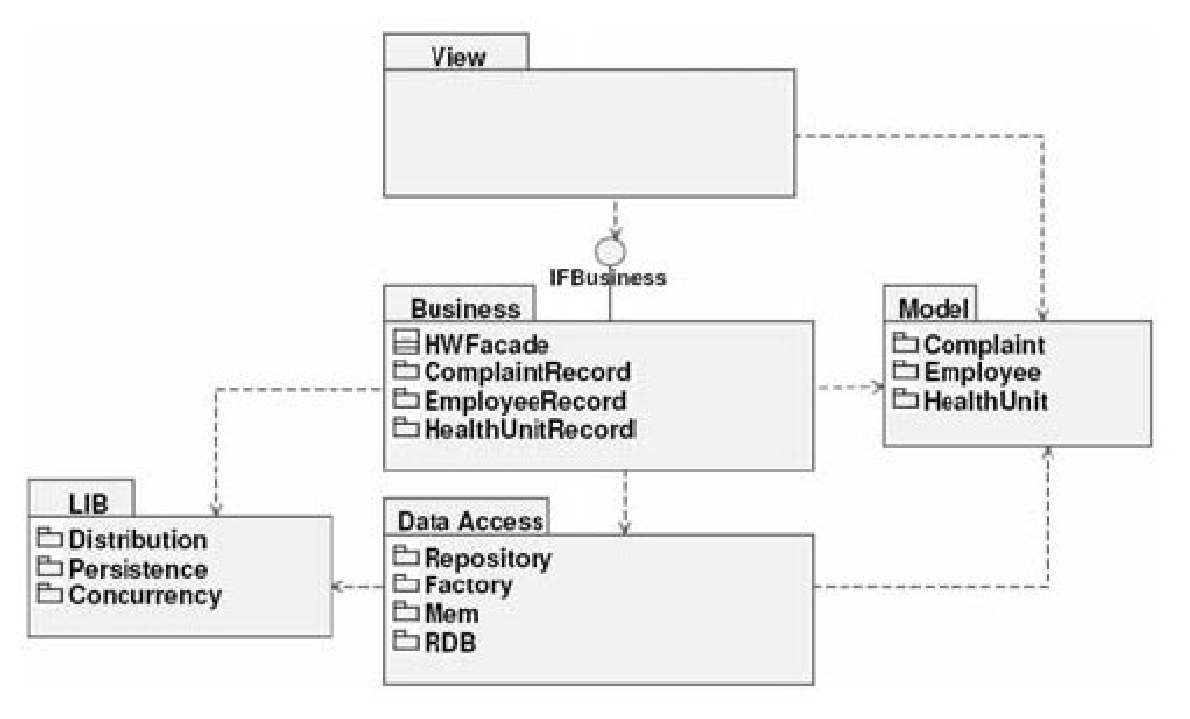
\includegraphics[scale=0.5]{images/hw.eps}
\caption{Overview of the Health Watcher architecture.}
\label{fig:hw-architecture}
\end{figure}

Figure~\ref{fig:hw-architecture} shows the base architecture of the
HW system. This architecture aims at modularizing user interface,
distribution, business rules, and data management concerns. Below
we describe the major architectural components of the HW system:

\begin{description}

\item [View Layer:] related with the HW web interface. The
implementation of this layer is based on Front
Controller~\cite{alur-book-2003} and
Command~\cite{gamma-dpbook-1995} patterns, using \emph{servlets}
and \emph{plain Java objects}. The communication with the business layer
is implemented with calls to the \emph{IFBusiness}, which may be
distributed or not.

\item [Business Layer:] responsible for business
logic and transactional concern implementation. The
\emph{HWFacade}, which implements \emph{IFBusiness}, is the unique
point of interaction with this layer. This class uses
\emph{record} components to interact with the Data Access Layer.

\item [Data Access Layer:] responsible for abstracting the persistence
mechanism following the Data Access Object
pattern~\cite{alur-book-2003}. Some interfaces to
manage data persistence are defined in this layer. Two
implementations are available: the first one uses volatile memory
whereas the second one is based on relational databases.

\item [Model:] responsible for implementing the \emph{domain objects}.
These objects represent the core concepts of the application;
transit between all architectural layers; and have a few
implementation logic. Complain, employee, and health unity are examples of 
core concepts in the HW system. 

\item [Lib Components:] represent reusable components that are useful
to the implementation of concerns like persistence, distribution,
and concurrency.
\end{description}

In what follows, we present several issues related to \emph{aspect-oriented} 
modularity. First, we discuss about the problem of unanticipated changes 
in base code --- problem named as fragile pointcut in the \emph{aspect-oriented} community. After that, 
we argue that clear interfaces, for decoupling crosscutting code from base 
code, are necessary for developing different concerns in parallel.    

\subsection{Unanticipated Changes in Base Code}

Suppose the requirement of synchronizing (concurrency management)
all methods of a class. Such a requirement consists of encompassing
with synchronized blocks the bodies of all methods.
Listing~\ref{lst:ao-synchronizing} illustrates an implementation of
this concern in AspectJ applied to the \emph{EmployeeRepository}
class.

\scriptsize
\begin{lstlisting}[frame=single, caption={Aspect responsible for implementing the concurrency concern.},label=lst:ao-synchronizing, language=Java]
public aspect SynchronizationAspect {

    Object around(Object o): this(o)
            && execution(* EmployeeRepository.*(..)) {
        synchronized(o) {
            return proceed(o);
        }
    }
}
\end{lstlisting}
\normalsize

Now, suppose a new feature intended to count the number of employees
registered in a given profile. Such a feature might be implemented as
a new method in the \emph{EmployeeRepository} class
(Listing~\ref{lst:new-method}).

\scriptsize
\begin{lstlisting}[frame=single, caption={A new method for counting the number of Employees.},label=lst:new-method, language=Java]
public class EmployeeRepository {

    public void insertEmployee(Employee employee) { ... }

    public void removeEmployee(Employee employee) { ... }

    public int getNumberOfEmployees(Profile profile) {
        // Business logic to count the number of Employees
    }

}
\end{lstlisting}
\normalsize

If a class developer oblivious about the
\emph{SynchronizationAspect} aspect decides to implement the
\emph{getNumberOfEmployees} method, at least three problems can
occur:

\begin{enumerate}

    \item the \emph{getNumberOfEmployees} method created by the class
    developer might not need concurrency management, but it will be
    synchronized by the aspect;

    \item if the class developer, oblivious about the aspect,
    implements concurrency management in the \emph{getNumberOfEmployees} method,
    such a method would be synchronized twice; and

    \item depending on how the synchronization approaches are implemented
    by the aspect and class developers, together they might lead the system
    to a dealock or a livelock situation~\cite{lea-java-coop-1999}.

\end{enumerate}

In such cases, the expected behavior of the system could be
compromised, since some additional synchronization would be created
or, even worst, the system might reach a dealock or a livelock.

The situation above exposes that problems of modularity have
occurred: (1) the comprehensibility is compromised, since two
modules should be studied in order to understand the concern; and
(2) the parallel development is problematic, because one developer
can implement unintended behavior into a module which, although it
is not under his responsibility, might break the system.

In summary, we conclude that any unanticipated change in the class
may cause problems and the application might not behave as presumed.
Notice that we have a cyclical dependency situation: the aspect
depends on the class syntactically; and to change the class, the
developer must be aware about the aspect.
Figure~\ref{dsm:concurrency} illustrates such a cyclical
dependency through a DSM (presented in Section~\ref{sec:software-modularity}), whereas
Figure~\ref{dsm:concurrency-drs} shows design rules coming into
play to remove the dependency between the aspect and class.

\begin{figure}[h]
    \begin{center}
        \subfigure[Cyclical Dependency between an aspect and a class.] {
            \begin{scriptsize}
            \begin{tabular}{|l|l|l|l|} \hline
                  &                             & 1     & 2     \\ \hline
                1 & SynchronizationAspect.aj    & \paintcell     & x     \\ \hline
                2 & EmployeeRepository.java     & x     & \paintcell      \\ \hline
            \end{tabular}
            \end{scriptsize}
            \label{dsm:concurrency}
        }
        \subfigure[Design Rules removing Cyclical Dependency.] {
            \begin{scriptsize}
            \begin{tabular}{|l|l|l|l|l|} \hline
                  &                             & 1     & 2    & 3 \\ \hline
                1 & Design Rules                &       &      &   \\ \hline
                2 & SynchronizationAspect.aj    & x     &      &   \\ \hline
                3 & EmployeeRepository.java     & x     &      &   \\ \hline
            \end{tabular}
            \end{scriptsize}
            \label{dsm:concurrency-drs}
        }
        \caption{Concurrency concern with/without Design Rules.}
    \end{center}
\end{figure}

\subsection{Unsupported Parallel Development}

Another example of modularity issue might arise when a team is
assigned to develop a crosscutting concern and another team is
assigned to develop the base concerns of a system. In order to
reduce the time-to-market, it may be desirable to develop both
concerns in parallel. However, without the use of a clear interface
between those concerns, a lot of communication might be required,
which, in fact, compromises the parallel development.

When reasoning about modularity in software engineering,
the benefit of parallel development is frequently not considered, even after
Parnas claimed that modularity is more than program structure. Actually,
his view regarding modularity is related to the assignment of development
activities, which, of course, may be reflected in the program
structure~\cite{parnas-icse-03}.

\begin{quote}\emph{
My early work clearly treated modularisation as a design
issue, not a language issue. A module was a work assignment,
not a subroutine or other language element. Although
some tools could make the job easier, no special tools were
needed to use the principal, just discipline and skill.}
(D. Parnas)
\end{quote}


% include the parnas review of modularity
% read a bit more about the steimann discussion on AOP modularity
% we need a clear interface for both aspect and base code....

A similar view of modularity was presented by Baldwin and
Clark~\cite{clark-design-rules-book},  since they
reported that a modular design reduces the communication paths among
design decisions, in such a way that unities of work can be developed
in parallel.

For instance, suppose that a team is responsible for developing
the use cases related to the \emph{complaint management} concern (a core concern
of Health Watcher system); and another team is responsible
for an auditing concern that must be triggered whenever a change in a
complaint occurs. Without a clear interface stating which are the relevant
complaint changes (the set of join-points) and how these join-points should be
written by the complaint management team, any increment in the core concern
must be communicated to the auditing team. Consequently, it is difficult to
implement the auditing concern at the same time that the complaint management
concern is being developed. Although these concerns can be encapsulated in
single unities, there is no modular design in this case.

For instance, consider the DSM depicted in Figure~\ref{dsm:hw01}, which represent
some design parameters and respective dependencies of the Health Watcher
system. Based on this DSM, we can realize that decisions regarded to the
complaint implementation (row 5) depends on decisions about complaint
requirements (dependency row 5, column 2), about architectural
decisions\footnote{Examples of architectural decisions for the Health Watcher
system are the selected style (layers), patterns, and technologies for each
layer or concern (presentation, distribution, persistence, and so on.)}
(dependency row 4, column 4), and about the auditing concern (dependency row 4,
column 6). This last dependency occurs because the team responsible for developing
the \emph{complaint concern} have to know how to develop the extension points for
the \emph{auditing concern}. Moreover, as we can observe in
Figure~\ref{dsm:hw01}, the auditing implementation also depends on the
complaint implementation decisions, since changes in its implementation should
be notified to the auditing implementation team. In this way, there is a
cyclical dependency between complaint implementation and auditing
implementation -- a clear example of non modular design.

\begin{figure}[htb]
\centering
\begin{scriptsize}
\begin{tabular}{|l|l|l|l|l|l|l|l|} \hline
  &                             & 1     & 2     & 3     & 4     & 5     & 6 \\ \hline
1 & Goals and constraints       &       &       &       &       &       &   \\ \hline
2 & Complaint requirements      & x     &       &       &       &       &   \\ \hline
3 & Auditing requirements       & x     &       &       &       &       &   \\ \hline
4 & Architectural decisions     & x     & x     &       &       &       &   \\ \hline
5 & Complaint implementation    &       & x     &       & x     &       & x \\ \hline
6 & Auditing AO implementation  &       &       & x     &       & x     &   \\  \hline
\end{tabular}
\end{scriptsize}
\caption{DSM Analysis Health Watcher}
\label{dsm:hw01}
\end{figure}


Based on the information hidden principle, we should encapsulate the
dependencies between complaint and auditing concerns in a special kind
of interface (a design rule). 
Applying design rules to our current example, we improve the design structure
by removing the cyclical dependencies between complaint and auditing concerns.
The reviewed DSM is presented in Figure~\ref{dsm:hw02}. Notice that a new parameter
(actually a design rule) was introduced (row 4) and all dependencies are bellow
the main diagonal (there is no more cyclical dependencies).

\begin{figure}[htb]
\centering
\begin{scriptsize}
\begin{tabular}{|l|l|l|l|l|l|l|l|l|} \hline
  &                                 & 1     & 2     & 3     & 4     & 5     & 6 & 7 \\ \hline
1 & Goals and constraints           &       &       &       &       &       &   &   \\ \hline
2 & Complaint requirements          & x     &       &       &       &       &   &   \\ \hline
3 & Auditing requirements           & x     &       &       &       &       &   &   \\ \hline
4 & Architectural decisions         & x     & x     &       &       &       &   &   \\ \hline
5 & Auditing design rule            &       & x     &   x   &       &       &   &   \\ \hline
6 & Complaint implementation        &       & x     &       &   x   & x     &   &   \\ \hline
7 & Auditing AO implementation      &       &       &   x   &       & x     &   &   \\ \hline
\end{tabular}
\end{scriptsize}
\caption{DSM Analysis Health Watcher}
\label{dsm:hw02}
\end{figure}

In order to improve the parallel development between class developers and 
aspect developers, it would be necessary to establish contracts for defining what 
is expected from both teams. Existing works, such as \emph{Open Modules}~\cite{aldrich-ecoop-05}, 
propose the use of interfaces for exposing \emph{joinpoints} in the base code, which, in fact, 
defines the responsibilities just for class developers, besides limiting the scope of advised code. 
Therefore, existing approaches do not offer mechanims for describing the responsibilities of aspect developers. 
As a consequence, class developers are still able to implement part of a concern 
assigned for a different team and they can not assume the existence 
of any behavior expected to be modularized as an aspect. 

For instance, consider the implementation of a mobile
game product line. Listing~\ref{lst:paint-method} presents part of 
a non-variant code responsible for painting graphical elements 
on the screen. Methods \emph{paintBeforeScrolling} and
\emph{paintScolling} are introduced (by means of intertype declararions),
and represent variation points that should be implemented as aspects for each 
target device. To our knowledge, there is no approach for specifying that such methods must be called 
within the \emph{paint} method and that they must be introduced by aspects. 

\scriptsize
\begin{lstlisting}[frame=single, caption={Dependency of a base code to an aspect code.},label=lst:paint-method, numbers=left, language=Java]
 public void paint(Graphics g) {
	Enemy myEnemy = null;
	int i = 0;
	int j = 0;
	g.setClip(0, 0, Resources.CANVAS_WIDTH, Resources.CANVAS_HEIGHT);
	paintBeforeScrolling(g);
	if (this.scroll.isScrolling) {
	 	paintScrolling(g);
	} else if (!isGameOver){
	 ...
\end{lstlisting}

\normalsize

TODO: Revisar o texto a seguir. A id�ia � simplific�-lo.

The Crosscut Programming Interfaces (XPIs) is one attempt for defining design rules between aspects and 
advised code~\cite{sullivan-sigsoft-2005,sullivan-ieee-sw-2006}. Such interfaces specify which are the exposed 
join-points of a base code. Although an abstract XPI representation was provided in~\cite{sullivan-sigsoft-2005}, Griswold et. al  
presented how to implement crosscutting interfaces as syntactic constructs of AspectJ~\citet{sullivan-ieee-sw-2006}. 
Based on this approach, design rules are documented using \emph{abstract pointcut descriptions} and constraints 
applied to the base code. These constraints might be written as \emph{declare warning} (or \emph{declare error}) constructs
or just as comments in the source code (when a constraint can not be expressed as a \emph{declare warning} 
or \emph{declare error}). 

XPIs authors argue that an important characteristic of their approach is that it does not require any new construct in 
the AspectJ language and there is no restriction to the pointcut visibility. In fact, this characteristic encourage the use of XPIs in environments that are already using the AspectJ language. However, most of the constraints required for defining the responsibilities of both 
class developers and aspect developers can not be checked using the proposed XPI language. Consequently, it is not possible 
to guarantee, at least automatically, if certain design rules are being obeyed. For instance, we can not express, using AspectJ constructs, 
that a call to a method \emph{must} occurs within the flow of another method. Actually, we can define such a pointcut, but if it does not exist,  no error is reported by the AspectJ compiler. Actually, pointcut constructs in AspectJ were proposed for specifying 
points of execution that should be augmented by advices. They were not proposed for specifying restrictions applied for base code developing. 

Aiming at specifying restrictions in base code using AspectJ like languages, developers are able to check if a {\bf non desirable} pointcut occurs in the source code (by means of \emph{declare error} or {declare warning} constructs). However, there is no construct which can be used for specifying that a specific pointcut {\bf must} occur in the source code. However, in order to improve modularity between crosscutting and base decisions, it is necessary to define what is expected from both teams (not only what aspect developers require, as supported by XPIs).   

Therefore, we propose a new design rule language that can be used for specifying interfaces between aspects and advised code. In what follows, 
we present the syntax and semantics of our proposed language. Then, in Section~\ref{}, we present an evaluation though different case studies. 